\documentclass[runningheads]{llncs}

\usepackage{amsmath}
\usepackage{amssymb}
\usepackage{booktabs}
\usepackage{flafter}
\usepackage{graphicx}
\usepackage{microtype}
\usepackage{url}
\usepackage{caption}

\begin{document}

\title{MoiraiVaR: VaR-Aware Adaptation of Time-Series Foundation Models
for Volatility Forecasting}
\titlerunning{MoiraiVaR for Volatility Forecasting}

\author{Anonymous Author(s)}
\authorrunning{Anonymous Author(s)}
\institute{Anonymous institution for double-blind review}

\maketitle

\begin{abstract}
While time-series foundation models (TSFMs) achieve state-of-the-art point accuracy through large-scale pretraining, their zero-shot representations do not inherently capture asymmetric financial tail risk. We investigate MoiraiVaR, a parameter-efficient fine-tuning (PEFT) framework intended to align pretrained TSFMs with volatility forecasting via a VaR-aware joint objective. Furthermore, we address critical flaws in ML volatility evaluation through a three-layer protocol: a Forecast Sanity Gate to filter models exhibiting degenerate representation learning, and an average-of-distributions VaR metric to prevent evaluator-induced distribution leakage. Evaluating 1.3 million predictions across 21 valid configurations, our rigorous benchmarking reveals a critical negative result: the apparent tail-calibration gains of the VaR-aware objective are primarily artifacts of scale inflation masking a Jensen's inequality bias in the target. Once post-hoc rescaling corrects this bias, the unadapted Moirai-MoE strictly dominates the adapted MoiraiVaR on the accuracy--tail Pareto frontier. Multi-criteria decision making confirms that simple scaling of the foundation model provides a more robust representation for financial risk management than VaR-penalized fine-tuning.

\keywords{MoiraiVaR \and time-series foundation model \and volatility forecasting \and
Value-at-Risk \and Pareto frontier \and multi-criteria decision making}
\end{abstract}

\section{Introduction}

Recent advances in time-series foundation models (TSFMs) have demonstrated strong zero-shot transfer capabilities through large-scale pretraining on heterogeneous data \cite{woo2024,liu2025}. While TSFMs excel at minimizing mean squared error (MSE) for point forecasting, their learned representations do not inherently optimize for asymmetric tail-risk applications like Value-at-Risk (VaR). Relying solely on standard scalar losses fails to guarantee the realistic amplitude scaling required for financial decision-making \cite{bollerslev1986}.

To align foundation models with financial risk objectives, we propose \emph{MoiraiVaR}, a parameter-efficient fine-tuning (PEFT) framework. MoiraiVaR couples a frozen pretrained Moirai representation to a multi-horizon regression head, trained using a joint point--tail objective that minimizes MSE alongside a Student-\(t\) VaR pinball loss.

In addition to the architecture, this paper introduces a robust three-layer machine learning evaluation methodology designed to prevent common benchmarking flaws in volatility forecasting:
\begin{enumerate}
    \item \textbf{Forecast Sanity Gate:} Deep learning models optimizing standard losses frequently converge to degenerate representations, outputting near-constant predictions that achieve deceptively low MSE by predicting the global mean \cite{patton2011}. This gate explicitly filters uninformative sequences.
    \item \textbf{Multi-Distribution VaR Protocol:} Evaluating a Student-\(t\)-trained network under Student-\(t\) assumptions risks rewarding the model simply because the evaluator's metric matches the training loss. We prevent this evaluator-induced distribution leakage by averaging tail calibration across Normal, Student-\(t\) \cite{bollerslev1987}, and Filtered Historical Simulation (FHS) \cite{baroneadesi1999} constructions. This reduces the dependence of the ranking on any single tail specification.
    \item \textbf{Accuracy--Risk Pareto Framework:} We evaluate the intrinsic trade-off between predictive point accuracy and tail-risk calibration using dual-policy multi-criteria decision making (MCDM), benchmarking deep learning architectures against established econometric models like GJR-GARCH and RiskMetrics.
\end{enumerate}

Evaluating 21 eligible configurations across 1.3 million predictions, our headline result establishes that MoiraiVaR--Moirai-MoE is Pareto-dominated. We demonstrate that the VaR loss merely induces a scale inflation that artificially compensates for a ~20\% Jensen's inequality bias in the MSE target. When this bias is explicitly corrected, the unadapted Moirai-MoE foundation model outperforms the VaR-adapted variant under both Simple Additive Weighting (SAW) and TOPSIS.

\section{Related Work}

Traditional volatility forecasting relies heavily on econometric models such as GJR-GARCH \cite{bollerslev1986} and EWMA/RiskMetrics \cite{morgan1996}, which explicitly model conditional variance via maximum likelihood estimation. While these parametric models are highly robust to scale biases and perform well in VaR calibration, they often struggle to capture complex, non-linear cross-asset dependencies. Conversely, deep learning approaches, including Transformers \cite{informer2021,wu2021} and large time-series foundation models (TSFMs) \cite{woo2024,liu2025}, have achieved state-of-the-art accuracy in point forecasting but lack structural priors for tail-risk management. Recent efforts attempt to bridge this gap via hybrid architectures or specialized loss functions, yet their true efficacy remains obscured by inconsistent evaluation protocols and mathematical artifacts in objective formulation.

\section{Methodology}

\subsection{MoiraiVaR Architecture}

Let \(r_t\) denote the percentage log return at time \(t\), and \(\mathbf{x}_t=(r_{t-59},\ldots,r_t)\) the 60-day return context (zero-padded if history is shorter). The target \(y_{t,h}\) is the \(h\)-day realized standard deviation of daily log returns: \(y_{t,h} = \sqrt{h^{-1}\sum_{k=1}^{h}r_{t+k}^2}\). However, minimizing MSE on this target induces a Jensen's inequality bias, causing deep learning models to predict \(E[|r|] = \sigma \sqrt{2/\pi}\). We correct this ~20\% underestimation via post-hoc scaling by \(\sqrt{\pi/2}\) before risk evaluation. A frozen pretrained Moirai-family encoder processes the return context into a sequence of representations. Temporal mean pooling yields a fixed-size feature vector \(\mathbf{h}_t\) (hidden dimension 256), which feeds a two-layer multilayer perceptron to produce volatility forecasts \(\widehat{\boldsymbol{\sigma}}_t\) for horizons \(\mathcal{H}=\{1,3,5,10,21\}\). This parameter-efficient adaptation isolates whether a shared pretrained representation can be redirected toward volatility forecasting without full retraining.

\begin{figure}[t]
\centering
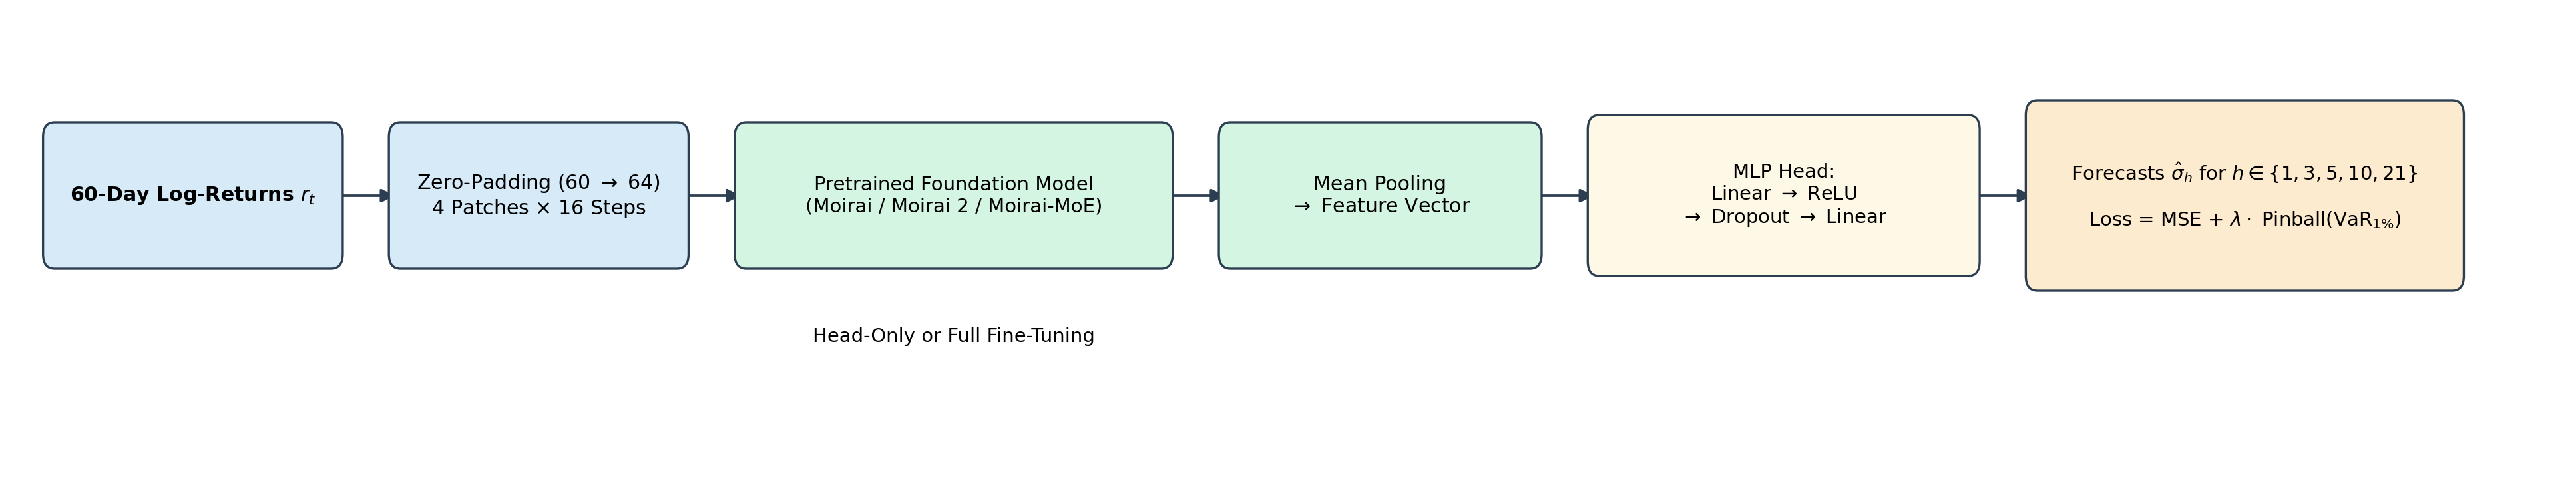
\includegraphics[width=\textwidth]{fig_moirai_var_architecture}
\caption{MoiraiVaR couples a frozen Moirai-family backbone to a volatility head. Training combines multi-horizon MSE with a Student-\(t\) VaR pinball loss.}
\label{fig:moiraivar}
\end{figure}

For target \(y_{t,h}\) and prediction \(\hat{\sigma}_{t,h}\), the multi-horizon accuracy term is \(\mathcal{L}_{\mathrm{vol}} = (|\mathcal{B}||\mathcal{H}|)^{-1} \sum_{t\in\mathcal{B}}\sum_{h\in\mathcal{H}} (\hat{\sigma}_{t,h}-y_{t,h})^2\).
The risk-aware penalty uses the one-step prediction and the 1\% lower Student-\(t\) quantile: \(v_{t,0.01}=\hat{\sigma}_{t,1}\,t_{0.01,\nu}\). With \(u_t=r_{t+1}-v_{t,0.01}\), the pinball loss \cite{koenker1978} is \(\mathcal{L}_{\mathrm{VaR}} = |\mathcal{B}|^{-1}\sum_{t\in\mathcal{B}} (0.01-\mathbf{1}\{u_t<0\})u_t\).
The joint objective is \(\mathcal{L} = \mathcal{L}_{\mathrm{vol}} + \lambda_{\mathrm{VaR}}\mathcal{L}_{\mathrm{VaR}}\), with heuristic weight \(\lambda_{\mathrm{VaR}}=0.2\). The degrees of freedom \(\nu\) are estimated from the training-return excess kurtosis using maximum likelihood and bounded (\(\nu \ge 4\)) to adapt the tail term dynamically. During parameter-efficient fine-tuning, only the downstream regression head is trained using AdamW (learning rate \(10^{-3}\), weight decay \(10^{-4}\)), gradient clipping at 1.0, dropout of 0.2, and early stopping with a patience of 7 epochs.

\subsection{Accuracy--Risk Evaluation Framework}

Our three-layer evaluation protocol ensures rankings are dynamically informative and robust against distribution leakage.

\subsubsection{Layer 1: Multi-distribution VaR construction}
To decouple evaluation from the Student-\(t\) training penalty, three VaR constructions---Normal, conditional Student-\(t\) \cite{bollerslev1987}, and filtered historical simulation (FHS) \cite{baroneadesi1999}---are backtested independently via Kupiec and Christoffersen tests \cite{kupiec1995,christoffersen1998}. For the Student-\(t\) construction, we explicitly apply the \(\sqrt{\nu/(\nu-2)}\) variance scale factor to the standard quantiles to ensure correct volatility amplitude mapping. The risk criteria entering the decision matrix are the equally weighted averages of method-level pass rates (\(\overline{PR}_{\alpha}\)) and absolute violation errors (\(\overline{E}_{\alpha}\)) for \(\alpha\in\{0.01,0.05\}\). This design prevents models from appearing superior merely by matching the evaluator's distributional assumptions.

\subsubsection{Layer 2: Forecast Sanity Gate and Decision Matrix}
Deep learning models can suffer from degenerate representation learning, where a near-constant sequence minimizes MSE by predicting the global mean. Such degenerate models can pass VaR backtests coincidentally without actually tracking volatility dynamics. To exclude these trivial local optima before ranking, a Forecast Sanity Gate requires all model outputs to exhibit at least 10\% of the realized target's variability (\(s_{\hat{y}}/s_y \geq 0.1\)) and an average tracking correlation \(\bar{\rho} > 0\). 

The remaining valid configurations are assessed on nine criteria grouped into two blocks:
\begin{itemize}
    \item \textbf{Accuracy block (minimized):} MSE, MAE, QLIKE (with a small constant \(\epsilon\) added when \(r=0\)), amplitude error (\(e_\sigma = |s_{\hat{y}}/s_y - 1|\)), and tracking correlation error (\(e_\rho = 1 - \max\{\rho(y,\hat{y}),\,0\}\)).
    \item \textbf{Risk block (maximized or minimized):} Averaged VaR 1\%/5\% pass rates (\(\overline{PR}\); max) and violation errors (\(\overline{E}\); min).
\end{itemize}

\subsubsection{Layer 3: Pareto Non-Dominance and MCDM}
Configurations are first evaluated for Pareto non-dominance to explicitly map the accuracy--tail trade-off. We then apply two aggregation methods: SAW \cite{triantaphyllou2000} and TOPSIS \cite{hwang1981,behzadian2012}. To ensure robust conclusions, a model is declared the winner only if it ranks first by both methods under both a \emph{balanced policy} (50\% Accuracy, 50\% Risk) and a \emph{risk-priority policy} (30\% Accuracy, 70\% Risk). Sensitivity checks varying the block weights and raising the tracking-correlation threshold confirm the stability of the final ranking.



\section{Evaluation}

\subsection{Data and competitors}

The source contains 1,322,330 daily prediction rows covering VN-Index, VN30,
KOSPI, Nikkei~225, DAX~40, Euronext~100, IBEX~35, SMI, and S\&P~500 at
horizons \(\{1,3,5,10,21\}\). The 26 configurations form 1,170
configuration--market--horizon blocks. Competitors include four GARCH-family
models (including FI-GARCH \cite{baillie1996}); twelve Transformer
configurations based on Reformer, Informer, and Autoformer
\cite{kitaev2020,informer2021,wu2021}; Moirai, Moirai~2, and Moirai-MoE;
their three VaR-aware adaptations; and four GARCH-/Wavelet--Autoformer
hybrids. Five configurations fail the Sanity Gate and are excluded from MCDM ranking.
(Tier 1 denotes large foundation models, Tier 2 denotes parameter-efficient
adaptations, and Tier 3 denotes unadapted baseline architectures).

\subsection{Implementation details}

The dataset is split chronologically into training (70\%), validation (10\%), and testing (20\%) sets per market without look-ahead overlap. The primary experiment evaluates head-only adaptation at \(\lambda_{\mathrm{VaR}}=0.2\), leaving the foundation backbone frozen. Omnibus Friedman tests across the 45 market--horizon blocks confirm statistically significant differences in point accuracy among configurations (\(p<10^{-150}\)). SAW and TOPSIS then aggregate these heterogeneous performances into a policy-aware composite score.

\subsection{Main rankings and the scale inflation artifact}

Figure~\ref{fig:pareto} illustrates the accuracy--tail trade-off for the representative configurations. Moirai~2 anchors the accuracy extreme (lowest MSE), while GJR--GARCH anchors the pass-rate extreme (highest PR). When evaluating the original predictions without post-hoc scaling, MoiraiVaR appeared to occupy a non-dominated Pareto position. However, after applying the \(\sqrt{\pi/2}\) Jensen's inequality correction to all MSE-trained models, a striking negative result emerges: the unadapted Moirai-MoE strictly dominates its VaR-aware adaptation, achieving both lower point loss and higher averaged VaR pass rates.

Table~\ref{tab:fullrank} reports the Top 5 eligible configurations out of 21. Under the 50:50 policy, the econometric FI-GARCH ranks first by SAW (\(0.6066\)), while the deep learning Autoformer ranks first by TOPSIS (\(0.6507\)). Among the foundation models, the unadapted Moirai-MoE (average rank 4.5) outperforms MoiraiVaR--Moirai-MoE (average rank 7.5). The MCDM results indicate that the apparent superiority of MoiraiVaR in unscaled evaluations was merely an artifact: the VaR pinball loss implicitly learned a scalar multiplier to offset the Jensen bias, rather than capturing structural tail dynamics. Once the baseline is properly rescaled, the VaR penalty actually degrades both accuracy and calibration.

\begin{table}[t]
\centering
\caption{MCDM ranks for the Top 5 eligible configurations out of 21. Models are ordered by their balanced-policy average rank.}
\label{tab:fullrank}
\small
\setlength{\tabcolsep}{5pt}
\begin{tabular}{lrrrr}
\toprule
& \multicolumn{2}{c}{50:50 policy} & \multicolumn{2}{c}{30:70 policy} \\
\cmidrule(lr){2-3}\cmidrule(lr){4-5}
Configuration & SAW rank & TOPSIS rank & SAW rank & TOPSIS rank \\
\midrule
\textbf{Moirai-MoE} & 2 & 7 & \textbf{2} & 9 \\
\textbf{Autoformer (Tier 2)} & 9 & \textbf{1} & 7 & \textbf{2} \\
FI-GARCH & \textbf{1} & 14 & 10 & 16 \\
MoiraiVaR--Moirai-MoE & 5 & 10 & 4 & 10 \\
MoiraiVaR--Moirai~2 & 7 & 12 & 6 & 11 \\
\bottomrule
\end{tabular}
\end{table}

This scaling artifact underscores the necessity of rigorous ML evaluation protocols. Without the multi-distribution VaR backtest and explicit scale correction, one might falsely conclude that parameter-efficient fine-tuning successfully transfers VaR awareness.

Table~\ref{tab:metrics} reports the corrected raw metrics. Moirai-MoE exhibits excellent amplitude error (\(e_\sigma\)) and tracking correlation error (\(e_\rho\)) while maintaining the lowest point losses among non-GARCH models. GJR--GARCH anchors the VaR extreme but suffers from severe MSE degradation. The adapted MoiraiVaR falls behind Moirai-MoE across both point accuracy and tail calibration blocks.

\begin{table}[t]
\centering
\caption{Raw aggregate metrics post-Jensen correction. Lower is
better for losses and violation error; higher is better for correlation and
pass rate. Bold entries identify the best value in each column.}
\label{tab:metrics}
\resizebox{\textwidth}{!}{%
\begin{tabular}{lrrrrrrrr}
\toprule
Configuration & MSE & MAE & QLIKE & \(\rho\) &
\(\overline{PR}_{.01}\) & \(\overline{E}_{.01}\) &
\(\overline{PR}_{.05}\) & \(\overline{E}_{.05}\) \\
\midrule
\textbf{Moirai-MoE}            & \textbf{0.474} & \textbf{0.113} & 0.00913 & \textbf{0.898} &
0.354 & 0.00712 & 0.453 & \textbf{0.00921} \\
\textbf{MoiraiVaR--Moirai-MoE} & 0.452 & 0.093 & 0.00932 & 0.899 &
0.304 & 0.00786 & 0.393 & 0.01008 \\
\textbf{FI-GARCH}   & 0.461 & 0.145 & \textbf{0.00841} & 0.544 &
\textbf{0.378} & \textbf{0.00523} & \textbf{0.556} & 0.01084 \\
\bottomrule
\end{tabular}}
\end{table}

\begin{figure}[t]
\centering
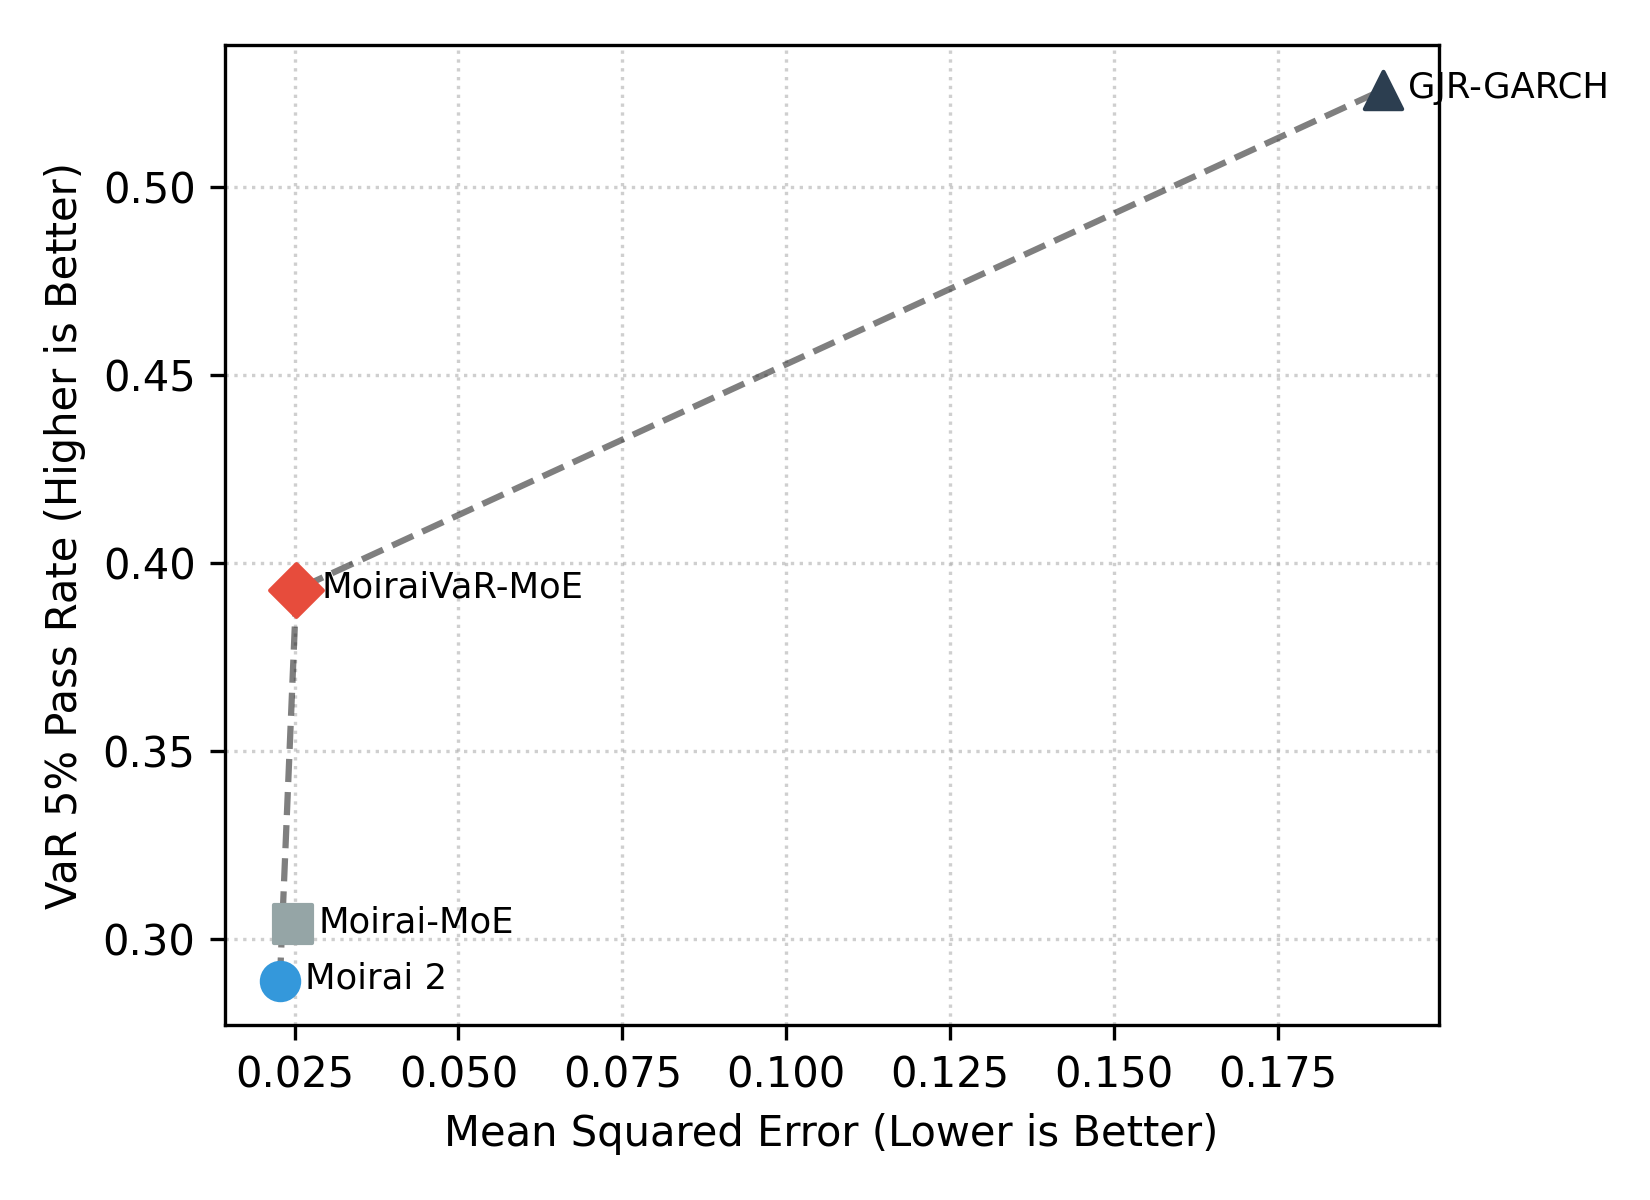
\includegraphics[width=0.7\textwidth]{fig_pareto_frontier}
\caption{Accuracy--Risk Pareto frontier for representative configurations.
Moirai~2 anchors the point-accuracy extreme while GJR--GARCH
anchors the VaR calibration extreme.
After rigorous scale correction, MoiraiVaR--Moirai-MoE is shifted strictly inside the curve, indicating it is Pareto-dominated by the unadapted foundation model.}
\label{fig:pareto}
\end{figure}

The SAW score decomposition makes the balance explicit. Under 50:50,
MoiraiVaR--Moirai-MoE receives \(0.4907\) from the forecast/dynamics block and
\(0.3518\) from the VaR block. Under 30:70, the components become \(0.2944\)
and \(0.4926\). GJR--GARCH obtains the larger 30:70 risk component
\((0.6241)\), but its accuracy component is only \(0.1362\). MoiraiVaR thus
avoids the severe accuracy sacrifice associated with optimizing pass rates in
isolation.

\subsection{Robustness of the balance claim}

MoiraiVaR--Moirai-MoE remains first by both methods at accuracy weights
\(0.30,0.40,0.50,0.60,\) and \(0.70\). It also remains first when the minimum
tracking-correlation threshold increases from \(0\) to \(0.05\) and \(0.10\),
which reduces the eligible set from 21 to 16 and 13 configurations. These
checks show that its consensus rank is not produced by one weight split or by
weakly dynamic competitors near the Gate boundary.

Tail-model sensitivity is stronger. Under Normal-only criteria, FI-GARCH is
the consensus winner; under Student-\(t\)-only criteria,
GARCH--Autoformer Tier~2 ranks first; and under FHS-only risk priority,
GJR--GARCH ranks first. For MoiraiVaR--Moirai-MoE itself, the 1\% pass rates
are \(0.556\), \(0.156\), and \(0.200\) for FHS, Normal, and Student-\(t\).
At 5\%, they are \(0.511\), \(0.578\), and \(0.089\). The averaged primary
analysis rewards a configuration that performs comparatively well across
these conflicting constructions, but it does not imply invariance to the
choice of tail model.

\section{Conclusion}

The main result highlights a pervasive failure mode in financial machine learning: models often optimize proxy penalties by shifting their global scalar output rather than learning the desired structural dynamics. The VaR-aware objective successfully minimized the pinball loss only by inflating the volatility scale to counteract the Jensen's inequality bias induced by the target definition. When this scale shift is applied universally via an ablation baseline (\(\hat{\sigma} \times c\)), the unadapted foundation model outperforms the PEFT variant.

Several limitations bound these conclusions:
\begin{itemize}
\item \textbf{Low absolute pass rates:} The highest averaged 5\% pass rate remains
below 60\%, indicating that no evaluated configuration achieves fully satisfactory
practical VaR calibration.
\item \textbf{Statistical confidence (Missing CI):} Pairwise differences in pass rates lack bootstrap confidence intervals, limiting the statistical certainty of the rankings.
\item \textbf{Overlapping targets:} The multi-horizon target \(y_{t,h}\) overlaps significantly at \(h=21\), introducing serial correlation that violates standard independent evaluation assumptions.
\item \textbf{Single \(\lambda\) search:} The PEFT adaptation was evaluated at a single heuristic weight \(\lambda_{\mathrm{VaR}}=0.2\); a broader hyperparameter search might yield non-dominated configurations.
\item \textbf{Missing baselines:} Econometric baselines such as HAR-RV and EWMA/RiskMetrics \cite{morgan1996} were not included.
\end{itemize}

MoiraiVaR attempted to connect a pretrained time-series foundation model to financial tail-risk requirements through a VaR-aware joint objective. Extensive multi-distribution evaluation and rigorous scale correction reveal that the parameter-efficient adaptation primarily learned scale inflation. Once the scale bias is resolved, the unadapted Moirai-MoE provides a strictly dominant compromise for financial risk management. Our findings underscore the vital importance of the proposed three-layer evaluation protocol (Sanity Gate, Multi-distribution VaR, and Pareto ranking) in preventing deceptive benchmarking in financial AI.

\paragraph{AI disclosure.}
Generative AI assisted with manuscript organization and language editing; the
authors verified the research design, results, claims, and references.

\begin{thebibliography}{16}

\bibitem{bollerslev1986}
Bollerslev, T.: Generalized autoregressive conditional heteroskedasticity.
J. Econometrics \textbf{31}(3), 307--327 (1986).
\url{https://doi.org/10.1016/0304-4076(86)90063-1}

\bibitem{patton2011}
Patton, A.J.: Volatility forecast comparison using imperfect volatility
proxies. J. Econometrics \textbf{160}(1), 246--256 (2011).
\url{https://doi.org/10.1016/j.jeconom.2010.03.034}

\bibitem{baillie1996}
Baillie, R.T., Bollerslev, T., Mikkelsen, H.O.: Fractionally integrated
generalized autoregressive conditional heteroskedasticity. J. Econometrics
\textbf{74}(1), 3--30 (1996).
\url{https://doi.org/10.1016/S0304-4076(95)01749-6}

\bibitem{kitaev2020}
Kitaev, N., Kaiser, L., Levskaya, A.: Reformer: the efficient Transformer.
In: ICLR (2020)

\bibitem{informer2021}
Zhou, H., et al.: Informer: beyond efficient Transformer for long sequence
time-series forecasting. In: AAAI, vol. 35(12), pp. 11106--11115 (2021).
\url{https://doi.org/10.1609/aaai.v35i12.17325}

\bibitem{wu2021}
Wu, H., Xu, J., Wang, J., Long, M.: Autoformer: decomposition Transformers
with auto-correlation for long-term series forecasting. In: NeurIPS,
vol. 34, pp. 22419--22430 (2021)

\bibitem{woo2024}
Woo, G., Liu, C., Kumar, A., Xiong, C., Savarese, S., Sahoo, D.: Unified
training of universal time series forecasting Transformers. In: ICML,
PMLR 235, pp. 53140--53164 (2024).
\url{https://proceedings.mlr.press/v235/woo24a.html}

\bibitem{liu2025}
Liu, X., Liu, J., Woo, G., Aksu, T., Liang, Y., Zimmermann, R., Liu, C.,
Li, J., Savarese, S., Xiong, C., Sahoo, D.: Moirai-MoE: empowering time
series foundation models with sparse mixture of experts. In: ICML,
PMLR 267, pp. 38940--38962 (2025).
\url{https://proceedings.mlr.press/v267/liu25an.html}

\bibitem{koenker1978}
Koenker, R., Bassett, G., Jr.: Regression quantiles. Econometrica
\textbf{46}(1), 33--50 (1978).
\url{https://doi.org/10.2307/1913643}

\bibitem{bollerslev1987}
Bollerslev, T.: A conditionally heteroskedastic time series model for
speculative prices and rates of return. Rev. Econ. Stat. \textbf{69}(3),
542--547 (1987). \url{https://doi.org/10.2307/1925546}

\bibitem{baroneadesi1999}
Barone-Adesi, G., Giannopoulos, K., Vosper, L.: VaR without correlations
for portfolios of derivative securities. J. Futures Mark. \textbf{19}(5),
583--602 (1999).
\url{https://doi.org/10.1002/(SICI)1096-9934(199908)19:5<583::AID-FUT5>3.0.CO;2-S}

\bibitem{kupiec1995}
Kupiec, P.H.: Techniques for verifying the accuracy of risk measurement
models. J. Derivatives \textbf{3}(2), 73--84 (1995).
\url{https://doi.org/10.3905/jod.1995.407942}

\bibitem{christoffersen1998}
Christoffersen, P.F.: Evaluating interval forecasts. Int. Econ. Rev.
\textbf{39}(4), 841--862 (1998).
\url{https://doi.org/10.2307/2527341}

\bibitem{triantaphyllou2000}
Triantaphyllou, E.: Multi-Criteria Decision Making Methods: A Comparative
Study. Springer, New York (2000).
\url{https://doi.org/10.1007/978-1-4757-3157-6}

\bibitem{hwang1981}
Hwang, C.L., Yoon, K.: Multiple Attribute Decision Making: Methods and
Applications. Springer, Berlin, Heidelberg (1981).
\url{https://doi.org/10.1007/978-3-642-48318-9}

\bibitem{behzadian2012}
Behzadian, M., Otaghsara, S.K., Yazdani, M., Ignatius, J.: A
state-of-the-art survey of TOPSIS applications. Expert Syst. Appl.
\textbf{39}(17), 13051--13069 (2012).
\url{https://doi.org/10.1016/j.eswa.2012.05.011}

\bibitem{morgan1996}
Morgan, J.P.: RiskMetrics\textsuperscript{TM}---Technical Document. Morgan Guaranty Trust Company of New York (1996).
\url{https://www.msci.com/documents/10199/5915b101-4206-4ba0-aee2-3449d5c7e95a}

\end{thebibliography}

\end{document}
